\chapter{Specifikacija programske potpore}
		
\section{Funkcionalni zahtjevi}

\noindent \textbf{Dionici:}
			
\begin{packed_enum}
	
	\item Vlasnik (naručitelj)
	\item Učenici				
	\item Korijenski administrator
	\item Administrator riječi
	\item Razvojni tim
	\item Neregistrirani korisnik
	
\end{packed_enum}

\noindent \textbf{Aktori i njihovi funkcionalni zahtjevi:}
			
			
\begin{packed_enum}
	\item  \underbar{Administrator riječi (inicijator) može:}
	
	\begin{packed_enum}
		
		\item pregledati i odabrati jezik te unutar tog jezika
		\begin{packed_enum}
			
			\item  stvoriti, urediti, brisati i pregledati riječi (riječ, opis, fraze, prijevod)
			\item  stvoriti, urediti, brisati i pregledati rječnike (naziv, broj riječi)
			\item dodati ili ukloniti riječ/i iz jednog ili više rječnika
	
		\end{packed_enum}
		
	\end{packed_enum}

	\item  \underbar{Korijenski administrator (inicijator) može:}
	
	\begin{packed_enum}
		
		\item stvoriti administratore riječi
		\item brisati administratore riječi
		\item sve što može i administrator riječi
		
	\end{packed_enum}

	\item \underbar{Učenik (inicijator) može:}
	
	\begin{packed_enum}

		\item pregledati i odabrati dostupne jezike
		\item pregledati i odabrati dostupne rječnike odabranog jezika
		\item započeti učenje odabirom jednog od četiri načina učenja
		\item izbrisati svoj korisnički račun 
	
	\end{packed_enum}

	\item  \underbar{Baza podataka (sudionik) može:}
	
	\begin{packed_enum}
		
		\item pohraniti sve podatke o učenicima i njihovim (ne)naučenim riječima
		\item pohraniti sve podatke o učenicima o administratorima 
		\item pohraniti sve podatke o riječima i rječnicima
		
	\end{packed_enum}

	\item  \underbar{API za rječnike (sudionik) može:}
	
	\begin{packed_enum}
		
		\item dohvatiti dodatne podatke o riječima (opis, fraza)
		
	\end{packed_enum}

	\item	\underbar{Neregistrirani korisnik (inicijator) može:}
	
	\begin{packed_enum}
		
		\item registrirati se:
		
		\begin{packed_enum}		
			
			\item potvrditi registraciju prijavom s inicijalnom lozinkom
			\item promijeniti inicijalnu lozinku
		
		\end{packed_enum}

	\end{packed_enum}

	\item	\underbar{Servis za ocjenu izgovora može:}
	
	\begin{packed_enum}
		
		\item ocijeniti korisnikov izgovor neke riječi ili izraza

	\end{packed_enum}

	\item	\underbar{Davatelj e-pošte može:}
	
	\begin{packed_enum}
		
		\item pruža uslugu stvaranja i korištenja e-mail računa

	\end{packed_enum}

\end{packed_enum}

\eject

\subsection{Obrasci uporabe}

\subsubsection{Opis obrazaca uporabe}

\noindent \underbar{\textbf{UC$<$broj obrasca$>$ - Prijava u sustav}}
\begin{packed_item}

	\item \textbf{Glavni sudionik: } Učenik ili administrator
	\item \textbf{Cilj: } Dobivanje pristupa učeničkom ili administratorskom sučelju
	\item \textbf{Sudionici: } Baza podataka
	\item \textbf{Preduvjet: } -
	\item  \textbf{Opis osnovnog tijeka:}
	
	\item[] \begin{packed_enum}

		\item Korisnik aplikacije unosi svoj e-mail i lozinku
		\item Sustav provjerava postoji li račun s istim podacima
		\item Ako su podaci ispravni, sustav preusmjerava korisnika na zaslon za odabir jezika (nastavak UC Pregledavanje i odabir jezika)

	\end{packed_enum}
	
	\item  \textbf{Opis mogućih odstupanja:}
	
	\item[] \begin{packed_item}

		\item[2.a] Neispravan e-mail ili lozinka
		\item[] \begin{packed_enum}
			
			\item Sustav obavještava korisnika o grešci
			
		\end{packed_enum}
		
	\end{packed_item}
\end{packed_item}


\noindent \underbar{\textbf{UC$<$broj obrasca$>$ - Pregledavanje i odabir jezika}}
\begin{packed_item}

	\item \textbf{Glavni sudionik: } Učenik ili administrator riječi
	\item \textbf{Cilj: } Odabrati željeni jezik iz popisa dostupnih jezika
	\item \textbf{Sudionici: } Baza podataka
	\item \textbf{Preduvjet: } UC Prijava u sustav
	\item  \textbf{Opis osnovnog tijeka:}
	
	\item[] \begin{packed_enum}

		\item Sustav korisniku prikazuje popis dostupnih jezika
		\item Korisnik odabire jezik
		\item Sustav preusmjerava:
		
		\item[] \begin{packed_item}

			\item učenika na zaslon za odabir rječnika (UC Pregledavanje i odabir rječnika)
			\item administratora na zaslon za upravljanje riječima i rječnicima
		
		\end{packed_item}

	\end{packed_enum}
	
\end{packed_item}

\noindent \underbar{\textbf{UC$<$broj obrasca$>$ - Potvrda brisanja elementa}}
\begin{packed_item}

	\item \textbf{Glavni sudionik: } Učenik ili administrator
	\item \textbf{Cilj: } Upozoriti korisnika i potvrditi brisanje bilo kojeg elementa sustava
	\item \textbf{Sudionici: } Baza podataka
	\item \textbf{Preduvjet: } Pohranjen je identifikator elementa kojeg želimo izbrisati	
	\item  \textbf{Opis osnovnog tijeka:}
	
	\item[] \begin{packed_enum}

		\item Sustav korisniku prikazuje popis dostupnih jezika
		\item Korisnik odabire jezik
		\item Sustav preusmjerava:
		
		\item[] \begin{packed_item}

			\item Korisniku je prikazan dijaloški okvir s porukom upozorenja o posljedicama brisanja te gumbovima "Obriši" i "Odustani"
			\item Korisnik potvrđuje brisanje klikom na gumb "Obriši"
			\item Odabrani element briše se iz baze podataka
		
		\end{packed_item}

	\end{packed_enum}

	\item  \textbf{Opis mogućih odstupanja:}
	
	\item[] \begin{packed_item}

		\item[2.a] Korisnik odustaje od brisanja
		\item[] \begin{packed_enum}
			
			\item Odabrani element ne briše se iz baze podataka
			
		\end{packed_enum}
		
	\end{packed_item}
	
\end{packed_item}

\noindent \underbar{\textbf{UC$<$broj obrasca$>$ - Stvaranje riječi}}
\begin{packed_item}

	\item \textbf{Glavni sudionik: } Admin riječi (nadalje Radmin)
	\item \textbf{Cilj: } Mogućnost pregledavanja svih riječi za zadani jezik
	\item \textbf{Sudionici: } Baza podataka
	\item \textbf{Preduvjet: } Prijavljivanje u Radmin račun, odabran jezik, Radmin se nalazi na stranici za pregled riječi (UC stvaranje riječi)	
	\item  \textbf{Opis osnovnog tijeka:}
	
	\item[] \begin{packed_enum}
		
		\item Radmin odabire opciju dodavanja riječi u sustav
		\item Dobiva ekran na kojem se nalaze prostori za unos teksta
		\item Radmin unosi riječ, pri čemu pomaže API
		\item Radmin unosi prijevod riječi, pri čemu pomaže API
		\item Radmin unosi značenje riječi koju dobiva iz API-ja
		\item Radmin unosi pomoćnu frazu koju dobiva iz API-ja
		\item Radmin unosi zvučnu datoteku izgovora riječi na odabranom jeziku

	\end{packed_enum}
	
\end{packed_item}


\noindent \underbar{\textbf{UC$<$broj obrasca$>$ - Uređivanje riječi}}
\begin{packed_item}

	\item \textbf{Glavni sudionik: } Admin riječi (nadalje Radmin)
	\item \textbf{Cilj: } Mogućnost pregledavanja svih riječi za zadani jezik
	\item \textbf{Sudionici: } Baza podataka
	\item \textbf{Preduvjet: } Prijavljivanje u Radmin račun, postojanje riječi u sustavu, odabran jezik
	\item  \textbf{Opis osnovnog tijeka:}
	
	\item[] \begin{packed_enum}
		
		\item Radmin odabire opciju pregleda riječi
		\item Na ekranu mu se prikazuje lista svih riječi u odabranom jeziku koje se nalaze u sustavu (bazi podataka)
		\item Pored svake riječi postoji stavka "uredi"
		\item Radmin bira opciju uređivanja riječi te ide na stranicu za uređivanje
		\item Ima opciju promijeniti pisanje riječi, pomoćnu frazu ili audio zapis, značenje je fiksno (ako radmin želi promijeniti značenje, mora ili dodati novu riječ, ili obrisati postojeću. Opet, može se dogoditi da se značenje riječi promjeni u nešto što se već nalazi u bazi podataka, što bi softverski bilo teško provjeriti)
		\item Nakon napravljenih željenih promjena, radmin potvrdi svoj rad i vraća se na pregled riječi

	\end{packed_enum}
	
\end{packed_item}


\noindent \underbar{\textbf{UC$<$broj obrasca$>$ - Pregledavanje riječi}}
\begin{packed_item}

	\item \textbf{Glavni sudionik: } Admin riječi (nadalje Radmin)
	\item \textbf{Cilj: } Mogućnost pregledavanja svih riječi za zadani jezik
	\item \textbf{Sudionici: } Baza podataka
	\item \textbf{Preduvjet: } Prijavljivanje u Radmin račun, postojanje riječi u sustavu, odabran jezik
	\item  \textbf{Opis osnovnog tijeka:}
	
	\item[] \begin{packed_enum}
		
		\item Radmin odabire opciju pregleda riječi
		\item Na ekranu mu se prikazuje lista svih riječi u odabranom jeziku koje se nalaze u sustavu (bazi podataka)

	\end{packed_enum}
	
\end{packed_item}

\noindent \underbar{\textbf{UC$<$broj obrasca$>$ - Stvaranje rječnika}}
\begin{packed_item}

	\item \textbf{Glavni sudionik: } Administrator riječi
	\item \textbf{Cilj: } Dodati novi rječnik u odabrani jezik
	\item \textbf{Sudionici: } Baza podataka
	\item \textbf{Preduvjet: } UC Pregledavanje i odabir rječnika
	\item  \textbf{Opis osnovnog tijeka:}
	
	\item[] \begin{packed_enum}
		
		\item Administratoru je prikazan obrazac za stvaranje rječnika
		\item Administrator upisuje naziv rječnika i potvrđuje unos
		\item Rječnik se dodaje u bazu podataka

	\end{packed_enum}

	\item  \textbf{Opis mogućih odstupanja:}
	
	\item[] \begin{packed_item}

		\item[2.a] Administrator je upisao prazan naziv rječnika
		\item[] \begin{packed_enum}
			
			\item Sustav javlja administratoru da naziv rječnika ne smije biti prazan
			
		\end{packed_enum}
		
	\end{packed_item}

\end{packed_item}

\noindent \underbar{\textbf{UC$<$broj obrasca$>$ - Promjena naziva rječnika}}
\begin{packed_item}

	\item \textbf{Glavni sudionik: } Administrator riječi
	\item \textbf{Cilj: } Promijeniti naziv odabranog rječnika
	\item \textbf{Sudionici: } Baza podataka
	\item \textbf{Preduvjet: } UC Pregledavanje i odabir rječnika
	\item  \textbf{Opis osnovnog tijeka:}
	
	\item[] \begin{packed_enum}
		
		\item Administrator u obrascu odabire opciju "Promijeni naziv"
		\item Administrator upisuje novi naziv i potvrđuje promjene
		\item Sustav sprema promjene u bazu

	\end{packed_enum}

	\item  \textbf{Opis mogućih odstupanja:}
	
	\item[] \begin{packed_item}

		\item[2.a] Administrator pokušava spremiti prazan naziv rječnika
		\item[] \begin{packed_enum}
			
			\item Sustav javlja administratoru da naziv rječnika ne smije biti prazan
			
		\end{packed_enum}

		\item[2.b] Administrator odustaje od promjena
		\item[] \begin{packed_enum}
			
			\item Promjene se ne spremaju u bazu
			
		\end{packed_enum}
		
	\end{packed_item}

\end{packed_item}

\noindent \underbar{\textbf{UC$<$broj obrasca$>$ - Promjena sadržaja rječnika}}
\begin{packed_item}

	\item \textbf{Glavni sudionik: } Administrator riječi
	\item \textbf{Cilj: } Izmjena popisa riječi u rječniku
	\item \textbf{Sudionici: } Baza podataka
	\item \textbf{Preduvjet: } UC Pregledavanje i odabir rječnika
	\item  \textbf{Opis osnovnog tijeka:}
	
	\item[] \begin{packed_enum}
		
		\item U obrascu je prikazan popis svih riječi u rječniku
		\item Administrator odabire opciju "Dodaj riječi"
		\item Administratoru je prikazan okvir s popisom svih riječi trenutnog jezika koje nisu u rječniku
		\item Administrator odabire jednu ili više riječi
		\item Administrator potvrđuje odabir
		\item Odabrane riječi dodaju se u rječnik

	\end{packed_enum}

	\item  \textbf{Opis mogućih odstupanja:}
	
	\item[] \begin{packed_item}

		\item[2.a] Administrator pokraj već dodane riječi odabire opciju "Ukloni riječ"
		\item[] \begin{packed_enum}
			
			\item Prikazuje se okvir za potvrdu brisanja (nastavak UC Potvrda brisanja elementa)
			\item Koraci 3.-6. se preskaču
			
		\end{packed_enum}

		\item[3.a] Sve su riječi odabranog jezika u odabranom rječniku
		\item[] \begin{packed_enum}
			
			\item Administratoru je prikazana informativna poruka umjesto popisa
			\item Administrator odustaje od mijenjanja rječnika
			\item Koraci 4.-6. se preskaču
			
		\end{packed_enum}

		\item[5.a] Administrator odustaje od promjena
		\item[] \begin{packed_enum}
			
			\item Promjene se ne spremaju u bazu
			
		\end{packed_enum}
		
	\end{packed_item}

\end{packed_item}
					

\noindent \underbar{\textbf{UC$<$broj obrasca$>$ - Brisanje rječnika}}
\begin{packed_item}

	\item \textbf{Glavni sudionik:} Administrator riječi
	\item  \textbf{Cilj:} Brisanje rječnika iz sustava
	\item  \textbf{Sudionici:} Baza podataka
	\item  \textbf{Preduvjet:} UC Pregledavanje i odabir rječnika
	\item  \textbf{Opis osnovnog tijeka:}
	
	\item[] \begin{packed_enum}

		\item Administrator potvrđuje brisanje rječnika $($UC Potvrda brisanja elementa$)$
		\item Sustav iz baze briše odabrani rječnik
	\end{packed_enum}

\end{packed_item}

\noindent \underbar{\textbf{UC$<$broj obrasca$>$ - Stvaranje administratora riječi}}
\begin{packed_item}

	\item \textbf{Glavni sudionik:} korijenski administrator
	\item  \textbf{Cilj:} Stvaranje admina riječi
	\item  \textbf{Sudionici:} Baza podataka
	\item  \textbf{Preduvjet:} Prijava korijenskog administratora u sustav $($UC Prijava u sustav$)$
	\item  \textbf{Opis osnovnog tijeka:}
	
	\item[] \begin{packed_enum}

		\item Korijenski administrator $($nadalje kAdmin$)$ odabire opciju ”stvori admina riječi”
		\item kAdmin dolazi na stranicu u kojoj mora upisati email adresu i lozinku novog admina riječi $($nadalje rAdmin$)$
		\item kAdmin potvrđuje stvaranje novog rAdmina
		\item Podaci se spremaju u bazu podataka
	\end{packed_enum}
	
	\item  \textbf{Opis mogućih odstupanja:}
	
	\item[] \begin{packed_item}

		\item[2.a] kAdmin može upisati email adresu već postojećeg rAdmina
		\item[] \begin{packed_enum}
			
			\item Sustav ga upozorava da već postoji rAdmin s upisanom email adresom							
		\end{packed_enum}

		\item[2.b] kAdmin unosi email korisnika
		\item[] \begin{packed_enum}
			
			\item Sustav ga upozorava da korisnička adresa ne može bit iskorištena pri stvaranju rAdmina								
		\end{packed_enum}
		
	\end{packed_item}
\end{packed_item}

\noindent \underbar{\textbf{UC$<$broj obrasca$>$ - Brisanje administratora riječi}}
\begin{packed_item}

	\item \textbf{Glavni sudionik: }korijenski administrator
	\item  \textbf{Cilj:} Uklanjanje Admina riječi iz sustava
	\item  \textbf{Sudionici:} Baza podataka
	\item  \textbf{Preduvjet:} Prijavljen kAdmin u sustav $($UC Prijava u sustav$)$, postojanje
	rAdmina kojeg se želi izbrisati
	\item  \textbf{Opis osnovnog tijeka:}
	
	\item[] \begin{packed_enum}

		\item kAdmin odabire opciju ”pregled rAdmina” i prikazuje mu se popis rAdmina
		\item kAdmin za specifičnog rAdmina odabire opcije ”obriši rAdmina”
		\item Odabirom te opcije mu se nudi prozorčić za potvrdu $($nastavak UC Potvrda brisanja elementa$)$
	\end{packed_enum}
	
\end{packed_item}

\noindent \underbar{\textbf{UC$<$broj obrasca$>$ - Registracija učenika}}
\begin{packed_item}

	\item \textbf{Glavni sudionik:} Neregistrirani korisnik
	\item  \textbf{Cilj:} Stvaranje učeničkog računa
	\item  \textbf{Sudionici:} Baza podataka, davatelj e-pošte
	\item  \textbf{Preduvjet:} -
	\item  \textbf{Opis osnovnog tijeka:}
	
	\item[] \begin{packed_enum}

		\item Učenik odabire opciju ”Registracija”
		\item Učenik unosi ime, prezime, e-mail i potvrđuje prijavu
		\item Učenik se prijavljuje u sustav s generiranom lozinkom (UC Prijava u sustav)							
		\item Sustav učeniku prikazuje obrazac za promjenu inicijalne lozinke (nastavak UC Promjena inicijalne lozinke)
	\end{packed_enum}
	
	\item  \textbf{Opis mogućih odstupanja:}
	
	\item[] \begin{packed_item}

		\item[2.a]Učenik se pokušava registrirati e-mail adresom na koju je već prijavljen račun
		\item[] \begin{packed_enum}
			
			\item Sustav upozorava korisnika i onemogućuje mu registraciju							
		\end{packed_enum}

		\item[2.b] Učenik se pokušava registrirati nepostojećom e-mail adresom
		\item[] \begin{packed_enum}
			
			\item Sustav upozorava korisnika i onemogućuje mu registraciju 								
		\end{packed_enum}
		
	\end{packed_item}
\end{packed_item}

\noindent \underbar{\textbf{UC$<$broj obrasca$>$ - Promjena inicijalne lozinke}}
\begin{packed_item}

	\item \textbf{Glavni sudionik:} Učenik
	\item  \textbf{Cilj:} Stvaranje računa
	\item  \textbf{Sudionici:} Baza podataka
	\item  \textbf{Preduvjet:} UC Registracija učenika
	\item  \textbf{Opis osnovnog tijeka:}
	
	\item[] \begin{packed_enum}

		\item Učenik u obrascu dvaput unosi novu lozinku i potvrđuje unos
		\item Ako se lozinke podudaraju nova se lozinka sprema u bazu i označava da
		je inicijalna lozinka promijenjena
		\item Sustav preusmjerava korisnika na zaslon za odabir jezika (UC Pregledavanje i odabir jezika)
	\end{packed_enum}
	
	\item  \textbf{Opis mogućih odstupanja:}
	
	\item[] \begin{packed_item}

		\item[1.a]Učenik gasi aplikaciju
		\item[] \begin{packed_enum}
			
			\item Ponovnom prijavom u sustav korisniku je prikazan obrazac za promjenu lozinke						
		\end{packed_enum}

		\item[2.a] Lozinke se ne podudaraju
		\item[] \begin{packed_enum}
			
			\item Sustav upozorava učenika i traži ispravak unosa  								
		\end{packed_enum}
		
	\end{packed_item}
\end{packed_item}

\noindent \underbar{\textbf{UC$<$broj obrasca$>$ - Pregledavanje i odabir rječnika}}
\begin{packed_item}

	\item \textbf{Glavni sudionik: } Učenik ili administrator riječi
	\item \textbf{Cilj: } Odabrati rječnik iz popisa rječnika nekog jezika
	\item \textbf{Sudionici: } Baza podataka
	\item \textbf{Preduvjet: } UC Pregledavanje i odabir jezika, postoji barem jedan rječnik odabranog jezika
	\item  \textbf{Opis osnovnog tijeka:}
	
	\item[] \begin{packed_enum}
		
		\item Korisniku su prikazani svi rječnici u odabranom jeziku
		\item Korisnik odabire jedan od njih
		\item Sustav preusmjerava:
		\item[] \begin{packed_item}
		
			\item učenika na zaslon za odabir načina učenja (UC Odabir načina učenja)
			\item administratora na obrazac za uređivanje rječnika (UC Promjena naziva rječnika, UC Promjena sadržaja rječnika)
			
		\end{packed_item}

	\end{packed_enum}

	\item  \textbf{Opis mogućih odstupanja:}
	
	\item[] \begin{packed_item}

		\item[1.a] Ne postoji nijedan rječnik u odabranom jeziku
		\item[] \begin{packed_enum}
			
			\item Korisniku je prikazana informativna poruka
			\item Preskaču se koraci 2. i 3.
			
		\end{packed_enum}
		\item[2.a] Administrator odabire opciju "Obriši rječnik" (vidljivo samo administratorima) pokraj jednog od rječnika
		\item[] \begin{packed_enum}
			
			\item Administrator nastavlja s brisanjem rječnika (UC Brisanje rječnika)
			\item Preskače se korak 3.
			
		\end{packed_enum}
		\item[2.b] Administrator odabire opciju "Dodaj novi rječnik"
		\item[] \begin{packed_enum}
			
			\item Administrator nastavlja sa stvaranjem rječnika (UC Stvaranje rječnika)
			\item Preskače se korak 3.
			
		\end{packed_enum}
		
	\end{packed_item}
	
\end{packed_item}


\noindent \underbar{\textbf{UC$<$broj obrasca$>$ - Odabir načina učenja}}
\begin{packed_item}

	\item \textbf{Glavni sudionik: } Korisnik
	\item \textbf{Cilj: } Započeti dnevnu sesiju učenja u odabranom načinu
	\item \textbf{Sudionici: } -
	\item \textbf{Preduvjet: } Postojanje korisničkog računa, prijava u sustav s korisničkim računom, odabir jezika i riječnika (UC pregledavanje i odabir riječnika)
	\item  \textbf{Opis osnovnog tijeka:}
	
	\item[] \begin{packed_enum}
		
		\item Korisnik bira jedan od četiri gumba koji predstavljaju načine rada
		\item Nakon odabira, korisnika se redirektira na stranicu tog specifičnog
		načina rada te se otpočinje s učenjem

	\end{packed_enum}

	
\end{packed_item}


\noindent \underbar{\textbf{UC$<$broj obrasca$>$ - Prijevod strane riječi}}
\begin{packed_item}

	\item \textbf{Glavni sudionik: } Korisnik
	\item \textbf{Cilj: } Korisnik je naučio prijevod strane riječi ili izraza na hrvatski
	\item \textbf{Sudionici: } Baza podataka
	\item \textbf{Preduvjet: } Učenik je prijavljen, učenik je prethodno odabrao koji će jezik učiti, iz kojeg će rječnika učiti te je odabrao način učenja Prijevod strane riječi (UC Odabir načina učenja)
	\item  \textbf{Opis osnovnog tijeka:}
	
	\item[] \begin{packed_enum}
		
		\item Korisniku je prikazana riječ na stranom jeziku s nekoliko ponuđenih prijevoda na hrvatski
		\item Korisnik odabire jedan od ponuđenih prijevoda
		\item Sustav korisnika obavještava je li odabrao ispravan prijevod
		\item Sustav korisniku nudi nastavak učenja ili povratak na odabir načina učenja

	\end{packed_enum}

\end{packed_item}


\noindent \underbar{\textbf{UC$<$broj obrasca$>$ - Prijevod na strani jezik}}
\begin{packed_item}

	\item \textbf{Glavni sudionik: } Korisnik
	\item \textbf{Cilj: } Korisnik je naučio prijevod strane riječi ili izraza na hrvatski
	\item \textbf{Sudionici: } Baza podataka
	\item \textbf{Preduvjet: } Učenik je prijavljen, učenik je prethodno odabrao koji će jezik učiti, iz kojeg će rječnika učiti te je odabrao način učenja Prijevod na strani jezik (UC Odabir načina učenja)
	\item  \textbf{Opis osnovnog tijeka:} 
	
	\item[] \begin{packed_enum}
		
		\item Korisniku je prikazana riječ na hrvatskom s nekoliko ponuđenih prijevoda na strani jezik
		\item Korisnik odabire jedan od ponuđenih prijevoda
		\item Sustav korisnika obavještava je li odabrao ispravan prijevod
		\item Sustav korisniku nudi nastavak učenja ili povratak na odabir načina učenja

	\end{packed_enum}

\end{packed_item}


\noindent \underbar{\textbf{UC$<$broj obrasca$>$ - Prijevod zvučnog zapisa}}
\begin{packed_item}

	\item \textbf{Glavni sudionik: } Korisnik
	\item \textbf{Cilj: } Korisnik slušajući razumije strani jezik
	\item \textbf{Sudionici: } Baza podataka
	\item \textbf{Preduvjet: } Učenik je prijavljen, učenik je prethodno odabrao koji će jezik učiti, iz kojeg će rječnika učiti te je odabrao način učenja Prijevod zvučnog zapisa (UC odabir načina učenja)
	\item  \textbf{Opis osnovnog tijeka:} 
	
	\item[] \begin{packed_enum}

		\item Korisniku klikom na simbol zvučnika čuje riječ ili izraz na stranom jeziku
		\item Korisnik odabire jedan od ponuđenih prijevoda 
		\item Sustav korisnika obavještava je li odabrao ispravan prijevod
		\item Sustav korisniku nudi nastavak učenja ili povratak na odabir načina učenja

	\end{packed_enum}

\end{packed_item}


\noindent \underbar{\textbf{UC$<$broj obrasca$>$ - Snimanje izgovora}}
\begin{packed_item}

	\item \textbf{Glavni sudionik: } Korisnik
	\item \textbf{Cilj: } Korisnik pravilno izgovara riječi na stranom jeziku
	\item \textbf{Sudionici: } Baza podataka, Servis za ocjenu izgovora
	\item \textbf{Preduvjet: } Učenik je prijavljen, učenik je prethodno odabrao koji će jezik učiti, iz kojeg će rječnika učiti te je odabrao način učenja Snimanje izgovora (UC odabir načina učenja)
	\item  \textbf{Opis osnovnog tijeka:} 
	
	\item[] \begin{packed_enum}

		\item Korisniku je ponuđena riječ na stranom jeziku
		\item Korisnik pritiskom na simbol mikrofona započinje snimanje zvuka
		\item Korisnik izgovara ponuđenu riječ na stranom jeziku
		\item Korisnik pritiskom na simbol mikrofona završava snimanje zvuka
		\item Sustav pomoću servisa za ocjenu izgovora korisnika obavještava o kvaliteti njegova izgovora
		\item Sustav korisniku nudi nastavak učenja ili povratak na odabir načina učenja

	\end{packed_enum}

\end{packed_item}


\noindent \underbar{\textbf{UC$<$broj obrasca$>$ - Brisanje korisničkog računa}}
\begin{packed_item}

	\item \textbf{Glavni sudionik: } Učenik
	\item \textbf{Cilj: } Iz sustavske baze podataka obrisati sve zapise o 
	učeničkom računu i naučenim riječima
	\item \textbf{Sudionici: } Baza podataka
	\item \textbf{Preduvjet: } UC Prijava u sustav
	\item  \textbf{Opis osnovnog tijeka:} 
	
	\item[] \begin{packed_enum}

		\item Korisnik odabire opciju "obriši moj račun"
		\item Korisniku se prikazuje dijaloški okvir brisanja računa gdje mu se opisuje koji podatci će biti izbrisani i obavještava ga se da sve riječi koje je naučio će također biti obrisane (nastavak UC Potvrda brisanja elementa)
	
	\end{packed_enum}

\end{packed_item}

\eject


\subsubsection{Dijagrami obrazaca uporabe}

\begin{figure}[H]
	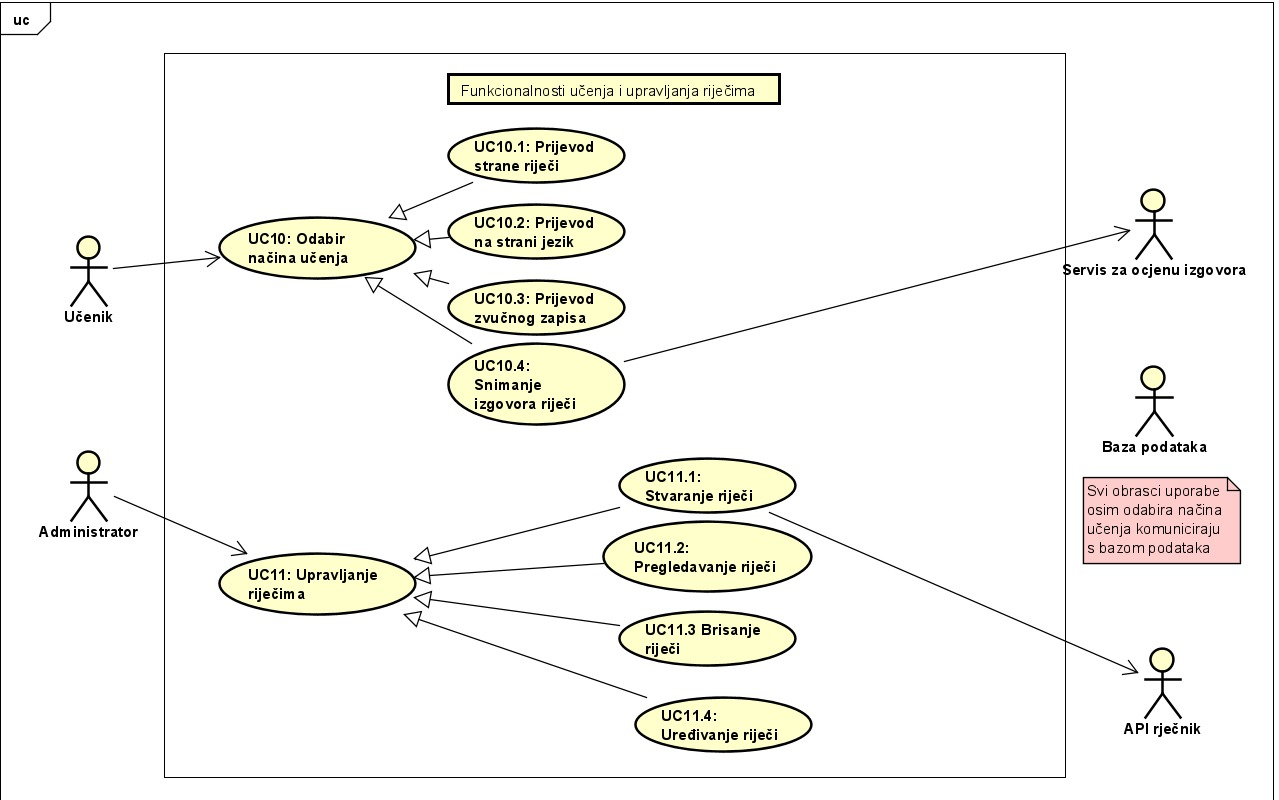
\includegraphics[scale=0.30]{dijagrami/dijagram1.jpg} 
	\centering
	\caption{Funkcionalnosti učenja i upravljanja riječima}
	\label{fig:dijagram1}
\end{figure}

\begin{figure}[H]
	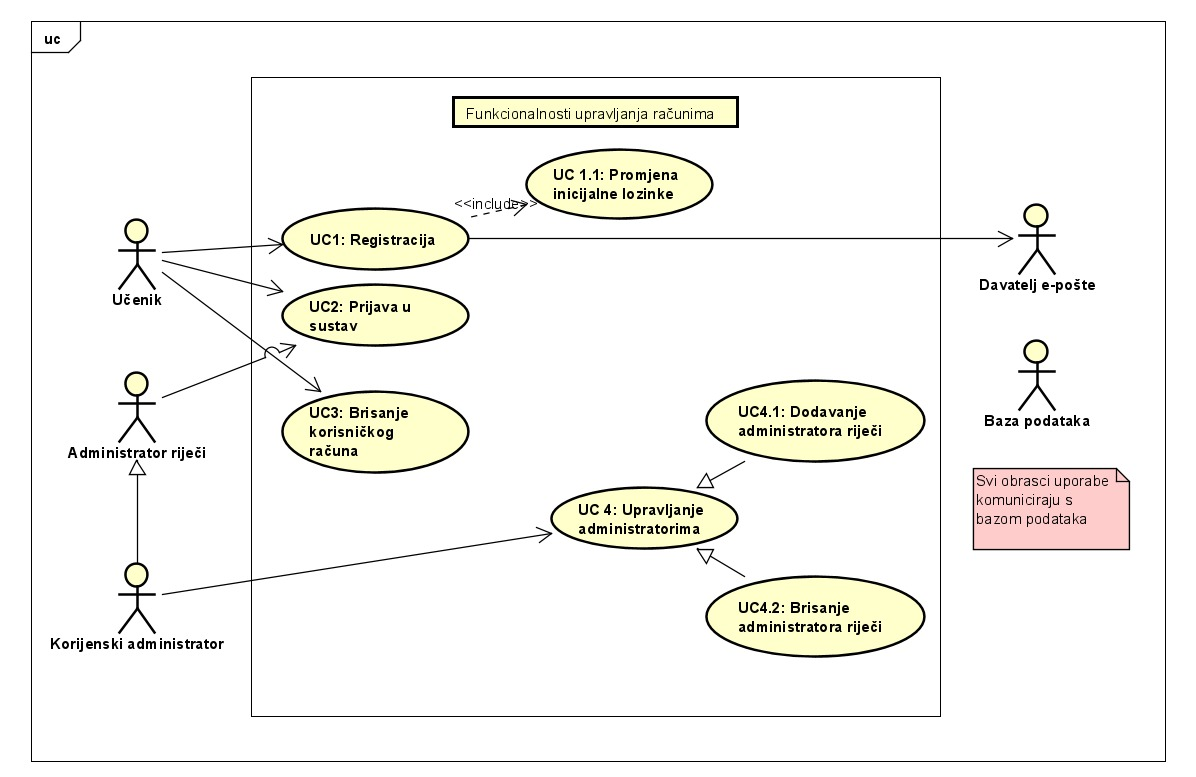
\includegraphics[scale=0.35]{dijagrami/dijagram2.jpg} 
	\centering
	\caption{Funkcionalnosti upravljanja računima}
	\label{fig:dijagram2}
\end{figure}

\begin{figure}[H]
	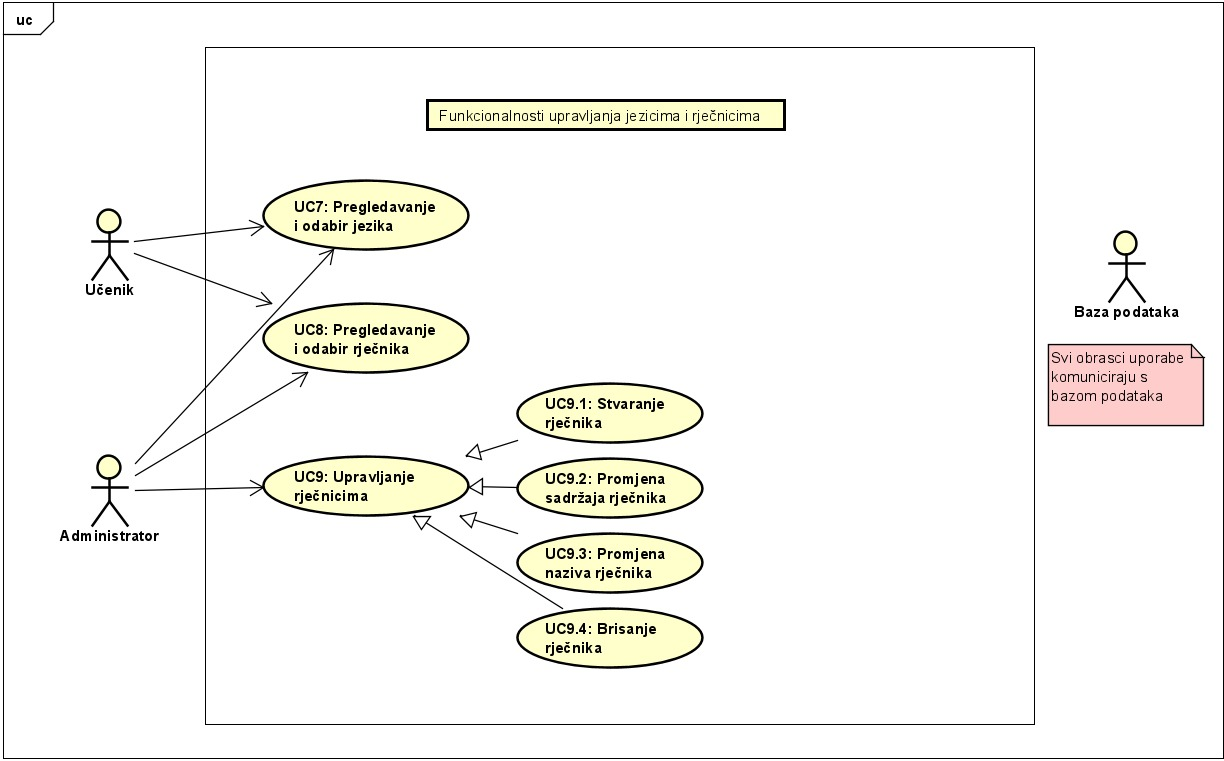
\includegraphics[scale=0.34]{dijagrami/dijagram3.jpg} 
	\centering
	\caption{Funkcionalnosti upravljanja jezicima i rječnicima}
	\label{fig:dijagram3}
\end{figure}	

\subsection{Sekvencijski dijagrami}

\textbf{\textit{dio 1. revizije}}\\

\textit{Nacrtati sekvencijske dijagrame koji modeliraju najvažnije dijelove sustava (max. 4 dijagrama). Ukoliko postoji nedoumica oko odabira, razjasniti s asistentom. Uz svaki dijagram napisati detaljni opis dijagrama.}
\eject

\section{Ostali zahtjevi}

\begin{itemize}
\item sustav korisniku daje povratnu informaciju o točnosti njegova odgovora
\item sustav u razumnom vremenu prezentira riječi nakon odabira načina rada
\item sustav mora imati potporu hrvatskih dijakritičkih znakova
\item sustavu iz javne mreže pristupamo protokolom HTTPS
\item sustav je dovoljno jednostavan i intuitivan za bilo koju dobnu skupinu korisnika 
\item za korištenje sustava korisniku je potrebno poznavanje hrvatskog jezika
\item rječnik mora imati barem 10 riječi
\item prijevodi riječi moraju biti ispravni
\end{itemize}
			 
			 
			 
	